\documentclass[palatino]{epflnotes}

\title{Mathematical modeling of DNA}
\author{Guillermo Julián Moreno}
\date{16/17 - Spring semester}

% Additional packages
\usepackage{siunitx}

% --------------------

\begin{document}
\frontmatter
\pagestyle{plain}
\maketitle

\tableofcontents
\mainmatter
% Content

\chapter{Introduction}

\section{Basics of dna}

The bases of DNA are denoted by $\mathcal{L} = \set{A,T,C,G}$ with a complementary  rule, where \begin{align*}
\conj{A} &= T &\conj{C} &= G \\
\conj{T} &= A &\conj{G} &= C
\end{align*}

An interesting? fact: the base of the DNA are antiparallel (orientation given by the orientation of the phosphate molecule).

The study of DNA can be separated in its three structures:
\begin{enumerate}
	\item The list of letters $x_i ∈ \mathcal{L} $ for $i = 1, \dotsc, 10^9$ (at least).
	\item The secondary structure is uniform: the double helix.
	\item The tertiary structure relates to the physical properties of the double helix, such as stiffness, which can vary greatly depending on the sequence (up to 25 \%), and its intrinsic shape (the shape of the central line).
\end{enumerate}

Molecular Dynamics simulations of the atoms in DNA and their surrounding medium (water) are considerably expensive, so the focus is in stochastic differential equations for which we can study output probability distribution.

The course-grained model implies simulating not all the atoms but only blocks (sugar, phosphate or whatever is a group for chemists), reducing thus the amount of degrees of freedom.

\section{Course-grained dna modeling}

We will be interested in models that predict the sequence ground-state structure and flexibility of a sequence. Each configuration space is a vector $w ∈ ℝ^N$ and the probability density function $ρ(w)$ depends on spome constants $Z,β$ and the free energy $U(w)$, so that \[ ρ(w) = \frac{1}{Z} e^{-βU(w)} \]

One special thing is four bases and not consider base pairs. ¿?

The set of parameters being modeled will by $6n$ intra-basepair and $6(n-1)$ inter-basepair degrees of freedom, so a totla of $N = 12n - 6$ degrees of freedom.

For the cgDNA model, the free energy is approximated as a quadratic form \[ U(w)= \frac{1}{2} (w - μ) · K(w -μ)\] with $μ = μ(S) ∈ ℝ^N$ being the ground state configuration and $K = K(S) ∈ ℝ^{N×N}$ being the ground-state stiffness, symmetric and positive-definite.

Of course, the question is how to get those ground states $μ, K$ from the sequence $S$ you are studying. The main assumption is junction and intra-basepair interaction energies, as shown in \fref{fig:MovementsDNA}.

\begin{figure}[tbp]
\centering
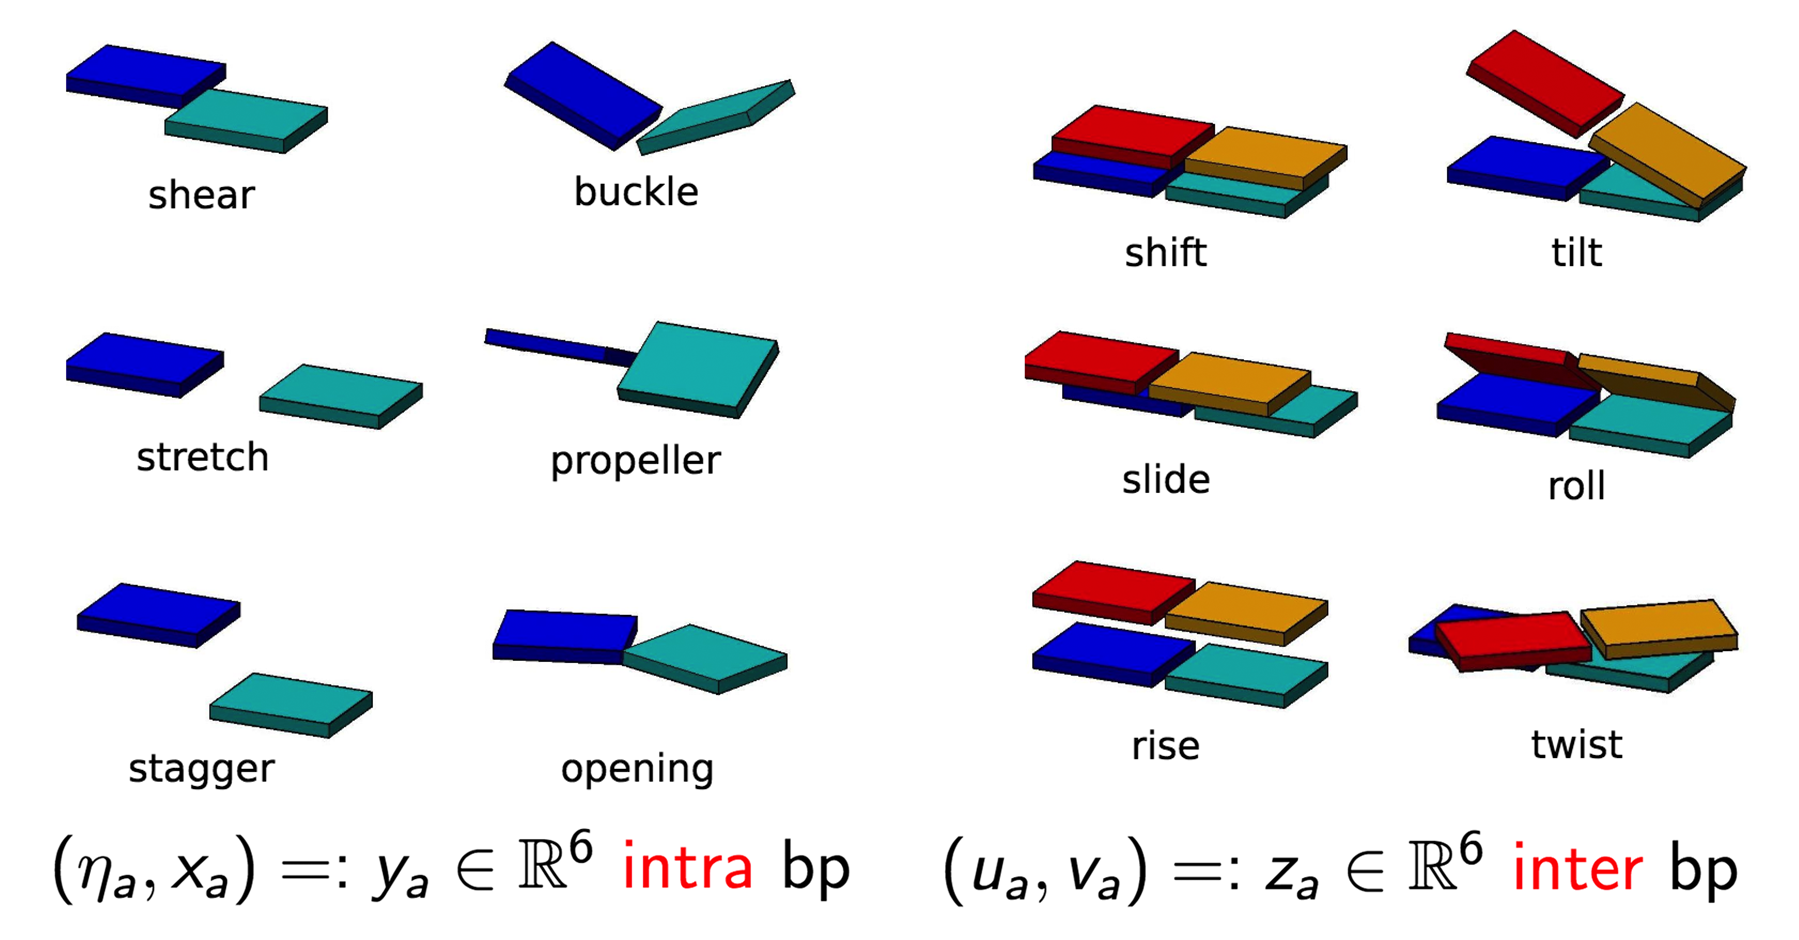
\includegraphics[width=0.8\textwidth]{img/movementsDNA.png}
\caption{Interpair and intrapair interactions}
\label{fig:MovementsDNA}
\end{figure}

\appendix

\chapter{Exercises}
% -*- root: ../MathModelingDNA.tex -*-

\backmatter
\printindex
\end{document}
